\part{Physik}
\section{Astronomie}
\section{Elektromagnetismus}
	\subsection{Elektromagnetische Welle}
		Als elektromagnetische Welle sind gekoppelte elektrischen und magnetischen Felder die sich im Raum mit Lichtgeschwindigkeit ausbreiten.
		\begin{figure}[h]
			\centering
			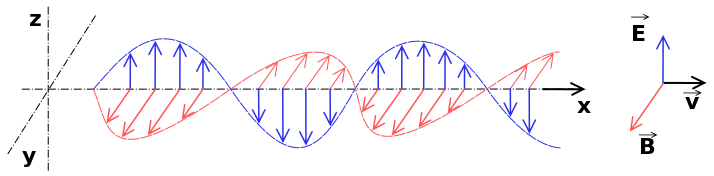
\includegraphics[width=0.8\linewidth]{./pics/ph/wave}
		\end{figure}
		\subsubsection*{Warum breitet sich eine elektromagnetische Welle aus?}
			Aus den mikroskopischen Maxwellgleichungen kann nachvollzogen werden wie J. C. Maxwell auf die Existenz der elektromagnetischen Welle gestoßen ist. Aus der ersten Feldgleichung wird geschlossen, dass ein sich zeitlich veränderndes Magnetfeld, von ringförmigen elektrischen Feldlinien umgeben ist.
			Er folgerte aus dem zweiten Maxwell'schen Feldgesetz: Während sich ein elektrisches Feld ändert, ist es von ringförmigen geschlossenen magnetischen Feldlinien umgeben.
			Somit also: Veränderliche elektrische Felder erzeugen magnetische Wirbelfelder und veränderliche Magnetfelder erzeugen elektrische Wirbelfelder.
			Es ergibt sich also eine Kette von Veränderungen des elektrischen und magnetischen Feldes, die sich als selbstständiges Gebilde im Raum ausbreitet. Ladungen erzeugen elektrische Felder und Ströme erzeugen magnetische Felder.
			Das erste Feldgesetz erweitert diesen Zusammenhang mit Hilfe des zweiten Feldgesetzes nun zu einer beliebig langen Kette:
			\begin{center}
				\large \textbf{Q $ \rightarrow $ E $ \rightarrow $ B $ \rightarrow $ E $ \rightarrow $ ...\\
					\text{ }I  $ \rightarrow $ B $ \rightarrow $ E $ \rightarrow $ B $ \rightarrow $ ...}
			\end{center}
			Elektromagnetische Wellen sind stets Transversalwellen.
			\begin{figure}[h]
				\centering
				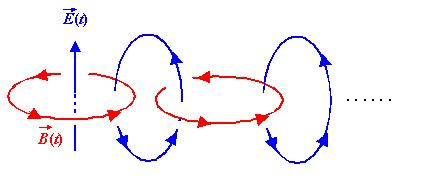
\includegraphics[width=0.3\linewidth]{./pics/ph/trans}
			\end{figure}
		\subsubsection{Quellen von elektromagnetische Wellen}
			\paragraph{Hertzscher Dipol}
				Ein hertzscher dipol ist eine Idealisierung eines Senders elektromagnetischer Strahlung und ist einem offenen elektrischen Schwingkreis äquivalent. Er dient somit als Grundlage für die Berechnung von Antennen.
				\begin{figure}[h]
					\centering
					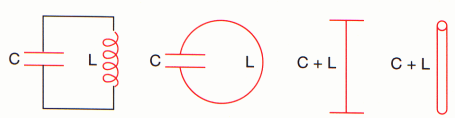
\includegraphics[width=0.6\linewidth]{./pics/ph/hertz}
					\caption{Transformation von einem Schwingkreis zum hertzschen Dipol}
				\end{figure}
				Bei der Transformation wird C und L immer kleiner, wodurch die Resonanzfrequenz steigt. Der hertzsche Dipol emittiert somit hochfrequente elektromagnetische Strahlung.
				\begin{figure}[h]
					\centering
					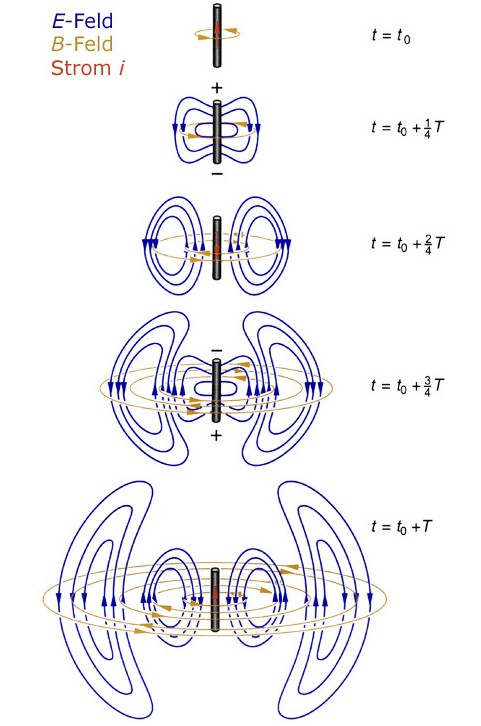
\includegraphics[width=0.4\linewidth]{./pics/ph/hertz2}
					\caption{Ausbreitung der elektromagnetischen Welle eines hertzschen Dipols}
				\end{figure}
			\paragraph{Röntgenstrahlung}
				Röntgenstrahlung kann durch zwei verschiedene Vorgänge entstehen:
				\begin{itemize}
					\item durch starke Beschleunigung geladener Teilchen (meistens Elektronen) -- dies ist die Bremsstrahlung, deren Spektrum kontinuierlich ist --
					\item und durch hochenergetische Übergänge in den Elektronenhüllen von Atomen oder Molekülen. Dies ist die charakteristische Röntgenstrahlung. Sie weist stets ein Linienspektrum auf.
				\end{itemize}
				\begin{tcolorbox}[title=Bremsstrahlung:]
					Wird eine elektrische Ladung beschleunigt, d.h. ändert sich ihr Geschwindigkeitsbetrag bzw. ihre Bewegungsrichtung, so entsteht elektromagnetische Strahlung. Die Energie der dabei auftretenden Photonen ist umso höher, je stärker die Beschleunigung ist.
				\end{tcolorbox}		
				Werden Elektronen auf eine Festkörperoberfläche beschleunigt und in diesem abgebremst, kommt es zu einer Beschleunigung (z.b. Richtungsänderung) durch etwa einen Atomkern. Diese Richtungsänderung führt nach obigem Satz zur Erzeugung von elektromagnetischen Wellen.\\
				Beide Effekte werden in der Röntgenröhre ausgenutzt, in der Elektronen zunächst von einer Glühwendel (Kathode) aus beschleunigt werden (dabei setzen sie keine Röntgenstrahlung frei, weil die Beschleunigung nicht groß genug ist) und anschließend auf die Anode treffen, in der sie stark abgebremst werden. Hierbei entsteht Röntgenstrahlung (Bremsstrahlung, mit insgesamt rund 1\% der eingestrahlten Energie) und Wärme (rund 99\%). Außerdem werden durch Elektronenstöße Elektronen aus den Schalen der Metallatome herausgeschlagen. 
				Ein Elektron wird z. B. durch einen Elektronenstoß aus der K-Schale entfernt und ein Elektron aus der L-Schale fällt in das Loch in der K-Schale. Die Energiedifferenz wird als charakteristische Röntgenstrahlung emittiert.
				\begin{figure}[h]
					\centering
					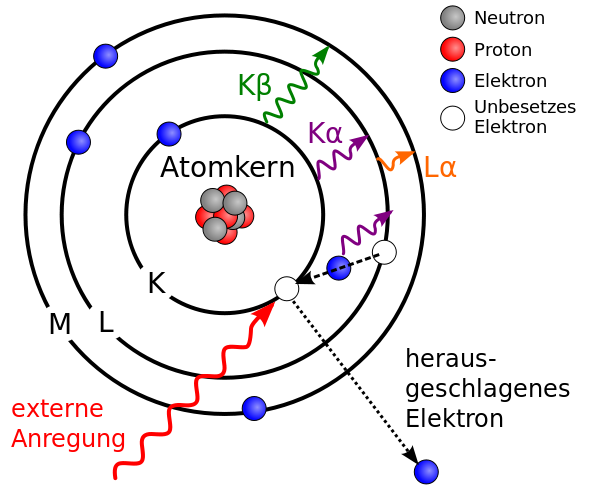
\includegraphics[width=0.4\linewidth]{./pics/ph/roentgen.png}
					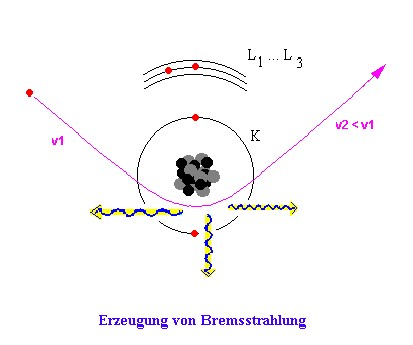
\includegraphics[width=0.4\linewidth]{./pics/ph/brems}
				\end{figure}
				Röntgenstrahlung ist ionisierend. Sie kann dadurch Veränderungen im lebenden Organismus hervorrufen und Schäden bis hin zu Krebs verursachen. Deshalb ist beim Umgang mit der Strahlung der Strahlenschutz zu beachten.
			\paragraph{Wärmestrahlung}	
				Genauso wie in Gasen und Flüssigkeiten eine thermische Molekularbewegung herrscht, haben auch die Atome von Festkörpern eine mirkoskopische kinetische bzw. potentielle Energie. Das heißt sie schwingen um ihre Ruhelagen. Diese mikroskopischen Energien nehmen mit steigender Temperatur zu und schwingen mit höheren Frequenzen. Durch dieses Schwingen von elektrischen Ladungen ändern sich die elektrischen Felder zwischen diesen Ladungen. Es resultiert ein elektrisches Wechselfeld, welches eine elektromagnetische Welle erzeugt, die sich in Form von Wärmestrahlung im Raum ausbreitet.\\
				Die Wärmestrahlung ist eine Art der Wärmeübertragung, bei der Energie anhand elektromagnetischer Wellen (infrarote Strahlung, infrarotes Licht) übertragen wird. Hierbei ist kein Trägermedium erforderlich, so dass also auch Wärme im Vakuum übertragen werden kann. Es ist aber eine direkte Sichtverbindung erforderlich, Hindernisse unterbrechen den Strahlungswärmeaustausch. Schwarze Körper absorbieren ein weites Spektrum an elektromagnetischen Wellen und reflektieren wenig, wodurch sie sich schneller als weiße Körper erwärmen, die mehr Strahlung reflektieren. Die physikalischen Eigenschaften des Materials bestimmen, welche Anteile einer auf das Bauteil auftreffenden Strahlung absorbiert, reflektiert oder transmittiert  werden.
			
				\begin{figure}[h]
					\centering
					\subfigure[Spektrale Energiedichte (abgestrahlte Energie je Wellenlänge) der Wärmestrahlung eines schwarzen Körpers bei verschiedenen Temperaturen]
					{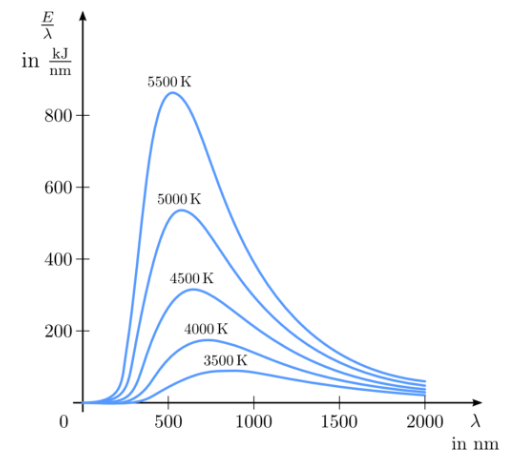
\includegraphics[width=0.45\textwidth]{./pics/ph/waermest}} \hspace{0.4cm}
					\subfigure[Beige Kurve entspricht der Temperatur der Sonne, Rote Kurve entspricht der Umgebungstemperatur] 
					{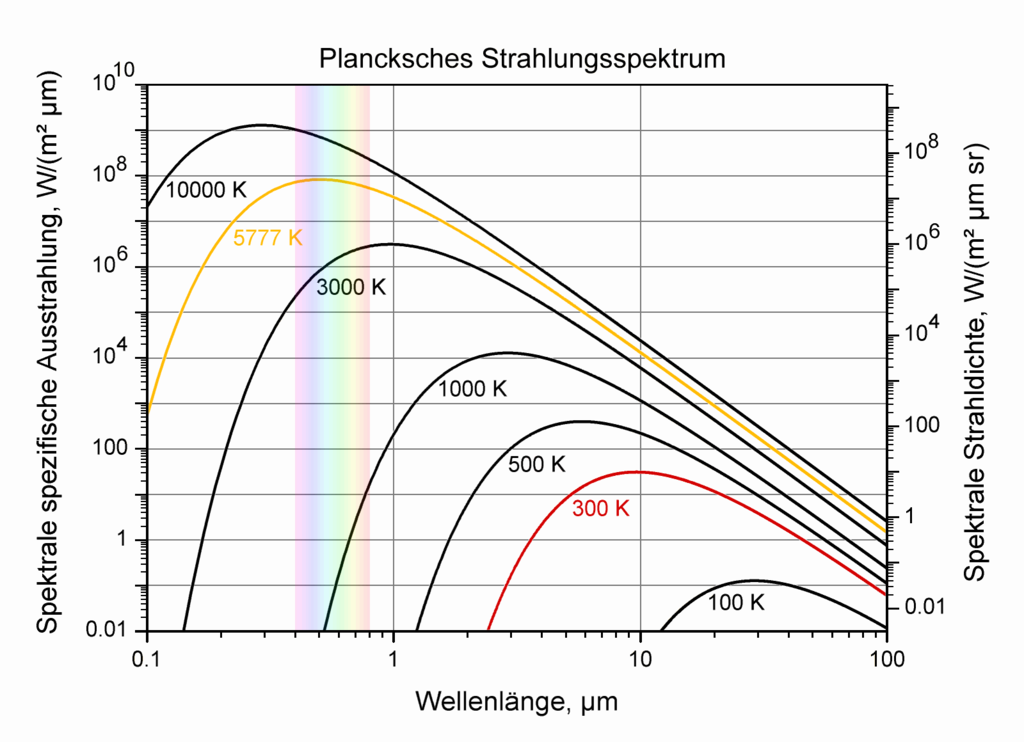
\includegraphics[width=0.45\textwidth]{./pics/ph/waremst}}
				\end{figure}
	\subsection{Welle-Teilchen-Dualismus}
		Der Welle-Teilchen-Dualismus ist eine Erkenntnis der Quantenphysik, wonach den Objekten der Quantenphysik gleichermaßen die Eigenschaften von Wellen, sowie die von  Teilchen zugeschrieben werden müssen. Je nach Art des Experiments tritt entweder der Wellen- oder der Teilchencharakter in Erscheinung, aber niemals beides gleichzeitig.
		\begin{itemize}
			\item Klassische Wellen breiten sich im Raum aus. Sie schwächen oder verstärken sich durch Überlagerung und können gleichzeitig an verschiedenen Stellen mit verschiedener Stärke einwirken.
			\item Ein klassisches Teilchen kann zu einem Zeitpunkt nur an einem bestimmten Ort anwesend sein. Nur dort wirkt es, aber stets mit seiner gesamten Energie, Ladung, Impuls etc.
		\end{itemize}
		Beide Eigenschaften scheinen sich gegenseitig auszuschließen. Trotzdem wurde in mehreren Schlüsselexperimenten für verschiedene Quantenobjekte belegt, dass beide Eigenschaften vorliegen, so dass man jedem Körper eine Materiewelle zuschreibt.\\\\
		Es ist unmöglich, eine anschauliche Vorstellung zu entwickeln, die dem Welle-Teilchen-Dualismus gerecht wird. Die Frage, ob beispielsweise Elektronen oder Lichtquanten „wirklich“ Teilchen oder Wellen seien, ist nicht zu beantworten. Sie sind vielmehr eine eigene Klasse von Quantenobjekten, die je nach der Art der Messung, die man an ihnen durchführt, entweder nur ihre Wellen- oder nur ihre Teilcheneigenschaft in Erscheinung treten lassen, aber nie beide gleichzeitig.\\\\
		Röntgen-, Gamma- und prinzipiell höher energetische Strahlung weist vorwiegend Teilchencharakter auf und niederenergetische Strahlung vorwiegend Wellencharakter.
		
	\subsection{Elektromagnetisches Spektrum}
		\begin{figure}[h]
			\centering
			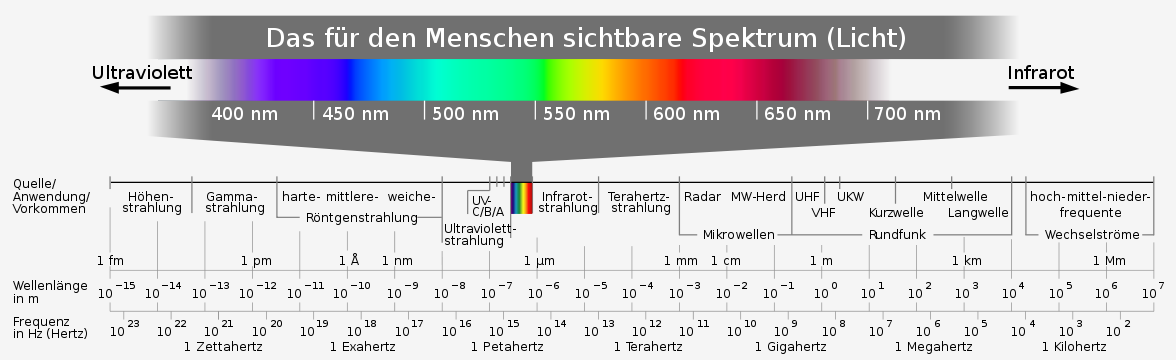
\includegraphics[width=1\linewidth]{./pics/ph/spektrum.png}
		\end{figure}
	